\documentclass{standalone}
\usepackage{tikz}
\usetikzlibrary{patterns, positioning}
\usepackage[sfdefault]{ClearSans} %% option 'sfdefault' activates Clear Sans as the default text font
\usepackage[T1]{fontenc}

\begin{document}
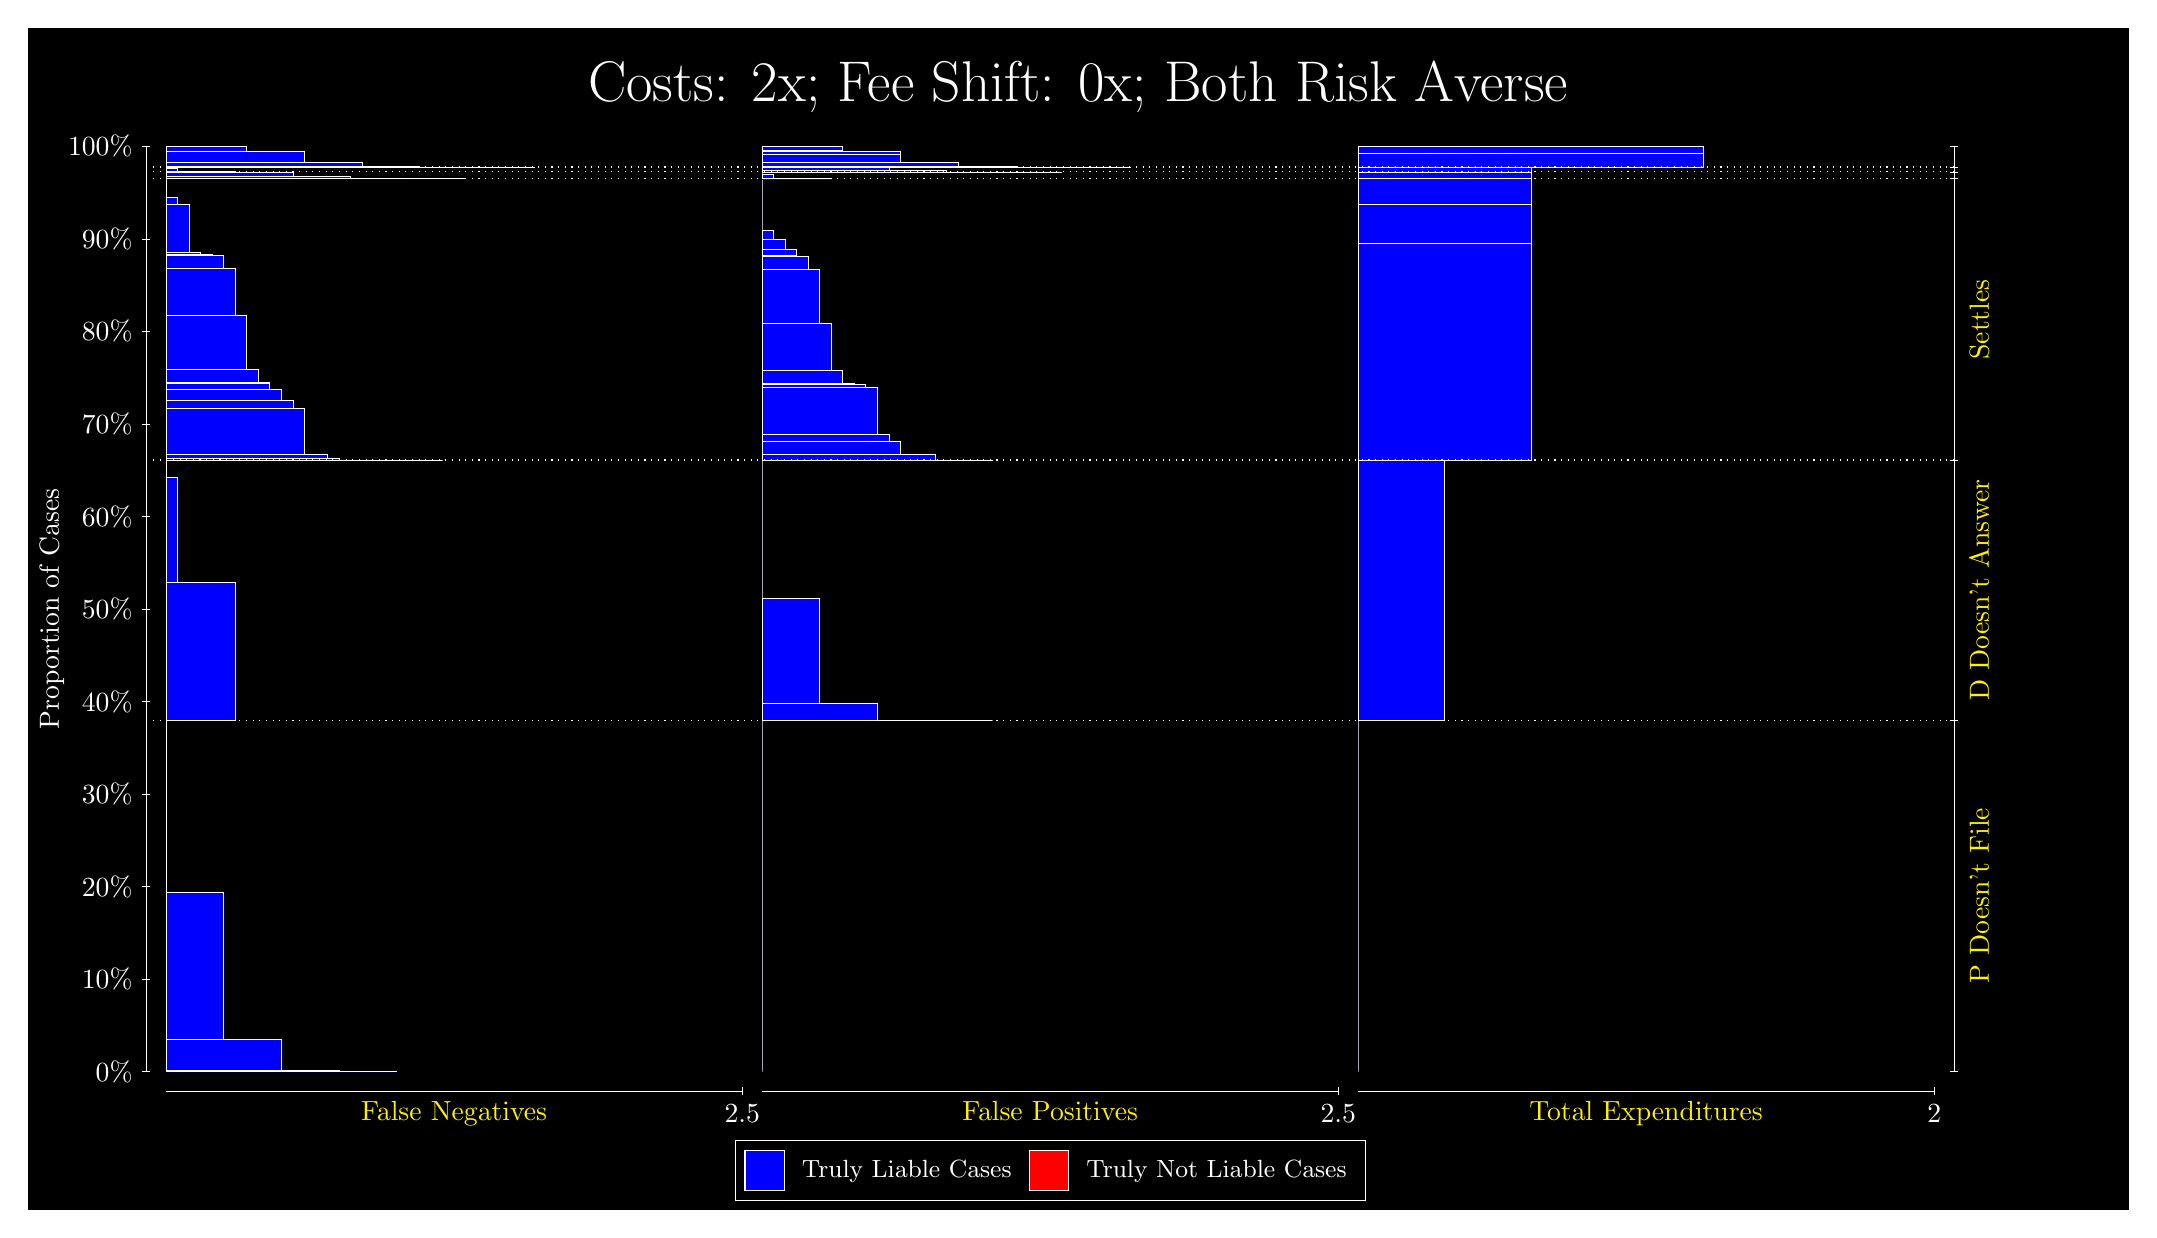
\begin{tikzpicture}
\draw[fill=black] (0,0) rectangle (26.667,15);
\draw[text=white] (0,13.5) rectangle (26.667,15) node[midway] {\huge Costs: 2x; Fee Shift: 0x; Both Risk Averse};
\draw[white, very thin] (1.5,1.75) -- (1.5,13.5);
\node[rotate=90, text=white, anchor=center] at (0.3, 7.625) {Proportion of Cases};
\draw[white, very thin] (1.45,1.75) -- (1.55,1.75);
\node[text=white, anchor=east] at (1.45, 1.75) {0\%};
\draw[white, very thin] (1.45,2.925) -- (1.55,2.925);
\node[text=white, anchor=east] at (1.45, 2.925) {10\%};
\draw[white, very thin] (1.45,4.1) -- (1.55,4.1);
\node[text=white, anchor=east] at (1.45, 4.1) {20\%};
\draw[white, very thin] (1.45,5.275) -- (1.55,5.275);
\node[text=white, anchor=east] at (1.45, 5.275) {30\%};
\draw[white, very thin] (1.45,6.45) -- (1.55,6.45);
\node[text=white, anchor=east] at (1.45, 6.45) {40\%};
\draw[white, very thin] (1.45,7.625) -- (1.55,7.625);
\node[text=white, anchor=east] at (1.45, 7.625) {50\%};
\draw[white, very thin] (1.45,8.8) -- (1.55,8.8);
\node[text=white, anchor=east] at (1.45, 8.8) {60\%};
\draw[white, very thin] (1.45,9.975) -- (1.55,9.975);
\node[text=white, anchor=east] at (1.45, 9.975) {70\%};
\draw[white, very thin] (1.45,11.15) -- (1.55,11.15);
\node[text=white, anchor=east] at (1.45, 11.15) {80\%};
\draw[white, very thin] (1.45,12.325) -- (1.55,12.325);
\node[text=white, anchor=east] at (1.45, 12.325) {90\%};
\draw[white, very thin] (1.45,13.5) -- (1.55,13.5);
\node[text=white, anchor=east] at (1.45, 13.5) {100\%};

\draw[white, very thin] (24.457,1.75) -- (24.457,13.5);
\draw[white, very thin] (24.407,1.75) -- (24.507,1.75);
\node[anchor=west] at (24.407, 1.75) {};
\draw[white, very thin] (24.407,6.2123) -- (24.507,6.2123);
\node[anchor=west] at (24.407, 6.2123) {};
\draw[white, very thin] (24.407,9.5158) -- (24.507,9.5158);
\node[anchor=west] at (24.407, 9.5158) {};
\draw[white, very thin] (24.407,13.088) -- (24.507,13.088);
\node[anchor=west] at (24.407, 13.088) {};
\draw[white, very thin] (24.407,13.176) -- (24.507,13.176);
\node[anchor=west] at (24.407, 13.176) {};
\draw[white, very thin] (24.407,13.238) -- (24.507,13.238);
\node[anchor=west] at (24.407, 13.238) {};
\draw[white, very thin] (24.407,13.5) -- (24.507,13.5);
\node[anchor=west] at (24.407, 13.5) {};

\draw[white, very thin, fill=blue] (1.75,1.75) rectangle (4.6775,1.7501);
\draw[white, very thin, fill=blue] (1.75,1.7501) rectangle (3.9457,1.7651);
\draw[white, very thin, fill=blue] (1.75,1.7651) rectangle (3.2138,2.1654);
\draw[white, very thin, fill=blue] (1.75,2.1654) rectangle (2.4819,4.0224);
\draw[white, very thin, fill=red] (1.75,4.0224) rectangle (1.75,4.0224);
\draw[white, very thin, fill=blue] (1.75,4.0224) rectangle (1.75,6.2123);
\draw[white, very thin, fill=blue] (1.75,6.2123) rectangle (2.6283,7.9675);
\draw[white, very thin, fill=blue] (1.75,7.9675) rectangle (1.8964,9.2976);
\draw[white, very thin, fill=red] (1.75,9.2976) rectangle (1.75,9.2976);
\draw[white, very thin, fill=blue] (1.75,9.2976) rectangle (1.75,9.5158);
\draw[white, very thin, fill=blue] (1.75,9.5158) rectangle (5.2631,9.5158);
\draw[white, very thin, fill=blue] (1.75,9.5158) rectangle (4.6775,9.5159);
\draw[white, very thin, fill=blue] (1.75,9.5159) rectangle (4.5312,9.5173);
\draw[white, very thin, fill=blue] (1.75,9.5173) rectangle (4.3848,9.5173);
\draw[white, very thin, fill=blue] (1.75,9.5173) rectangle (4.092,9.5175);
\draw[white, very thin, fill=blue] (1.75,9.5175) rectangle (3.9457,9.5327);
\draw[white, very thin, fill=blue] (1.75,9.5327) rectangle (3.7993,9.5871);
\draw[white, very thin, fill=blue] (1.75,9.5871) rectangle (3.6529,9.5949);
\draw[white, very thin, fill=blue] (1.75,9.5949) rectangle (3.5065,10.168);
\draw[white, very thin, fill=blue] (1.75,10.168) rectangle (3.3602,10.28);
\draw[white, very thin, fill=blue] (1.75,10.28) rectangle (3.2138,10.409);
\draw[white, very thin, fill=blue] (1.75,10.409) rectangle (3.0674,10.489);
\draw[white, very thin, fill=blue] (1.75,10.489) rectangle (3.0674,10.501);
\draw[white, very thin, fill=blue] (1.75,10.501) rectangle (2.921,10.664);
\draw[white, very thin, fill=blue] (1.75,10.664) rectangle (2.7746,11.349);
\draw[white, very thin, fill=blue] (1.75,11.349) rectangle (2.6283,11.952);
\draw[white, very thin, fill=blue] (1.75,11.952) rectangle (2.4819,12.11);
\draw[white, very thin, fill=blue] (1.75,12.11) rectangle (2.3355,12.129);
\draw[white, very thin, fill=blue] (1.75,12.129) rectangle (2.3355,12.129);
\draw[white, very thin, fill=blue] (1.75,12.129) rectangle (2.1891,12.158);
\draw[white, very thin, fill=blue] (1.75,12.158) rectangle (2.0428,12.765);
\draw[white, very thin, fill=blue] (1.75,12.765) rectangle (1.8964,12.855);
\draw[white, very thin, fill=red] (1.75,12.855) rectangle (1.75,12.855);
\draw[white, very thin, fill=blue] (1.75,12.855) rectangle (1.75,13.088);
\draw[white, very thin, fill=blue] (1.75,13.088) rectangle (5.5558,13.088);
\draw[white, very thin, fill=blue] (1.75,13.088) rectangle (4.8239,13.088);
\draw[white, very thin, fill=blue] (1.75,13.088) rectangle (4.092,13.121);
\draw[white, very thin, fill=blue] (1.75,13.121) rectangle (3.3602,13.175);
\draw[white, very thin, fill=blue] (1.75,13.175) rectangle (2.6283,13.176);
\draw[white, very thin, fill=red] (1.75,13.176) rectangle (1.75,13.176);
\draw[white, very thin, fill=blue] (1.75,13.176) rectangle (2.6283,13.177);
\draw[white, very thin, fill=blue] (1.75,13.177) rectangle (1.8964,13.215);
\draw[white, very thin, fill=red] (1.75,13.215) rectangle (1.75,13.215);
\draw[white, very thin, fill=blue] (1.75,13.215) rectangle (1.75,13.238);
\draw[white, very thin, fill=blue] (1.75,13.238) rectangle (6.4341,13.238);
\draw[white, very thin, fill=blue] (1.75,13.238) rectangle (5.7022,13.238);
\draw[white, very thin, fill=blue] (1.75,13.238) rectangle (4.9703,13.243);
\draw[white, very thin, fill=blue] (1.75,13.243) rectangle (4.2384,13.303);
\draw[white, very thin, fill=blue] (1.75,13.303) rectangle (3.5065,13.435);
\draw[white, very thin, fill=blue] (1.75,13.435) rectangle (2.7746,13.496);
\draw[white, very thin, fill=blue] (1.75,13.496) rectangle (2.0428,13.5);
\draw[white, very thin, fill=red] (1.75,13.5) rectangle (1.75,13.5);
\draw[white, very thin, fill=blue] (1.75,13.5) rectangle (1.75,13.5);
\draw[white, very thin, fill=red] (9.3189,1.75) rectangle (9.3189,1.75);
\draw[white, very thin, fill=blue] (9.3189,1.75) rectangle (9.3189,6.2123);
\draw[white, very thin, fill=red] (9.3189,6.2123) rectangle (12.246,6.2123);
\draw[white, very thin, fill=blue] (9.3189,6.2123) rectangle (12.246,6.2123);
\draw[white, very thin, fill=blue] (9.3189,6.2123) rectangle (11.515,6.2134);
\draw[white, very thin, fill=blue] (9.3189,6.2134) rectangle (10.783,6.4305);
\draw[white, very thin, fill=blue] (9.3189,6.4305) rectangle (10.051,7.7607);
\draw[white, very thin, fill=blue] (9.3189,7.7607) rectangle (9.3189,9.5158);
\draw[white, very thin, fill=red] (9.3189,9.5158) rectangle (12.246,9.5158);
\draw[white, very thin, fill=blue] (9.3189,9.5158) rectangle (12.246,9.516);
\draw[white, very thin, fill=red] (9.3189,9.516) rectangle (11.954,9.516);
\draw[white, very thin, fill=blue] (9.3189,9.516) rectangle (11.954,9.516);
\draw[white, very thin, fill=red] (9.3189,9.516) rectangle (11.661,9.516);
\draw[white, very thin, fill=blue] (9.3189,9.516) rectangle (11.661,9.5162);
\draw[white, very thin, fill=blue] (9.3189,9.5162) rectangle (11.515,9.5919);
\draw[white, very thin, fill=red] (9.3189,9.5919) rectangle (11.368,9.5919);
\draw[white, very thin, fill=blue] (9.3189,9.5919) rectangle (11.368,9.5921);
\draw[white, very thin, fill=blue] (9.3189,9.5921) rectangle (11.222,9.5922);
\draw[white, very thin, fill=red] (9.3189,9.5922) rectangle (11.075,9.5922);
\draw[white, very thin, fill=blue] (9.3189,9.5922) rectangle (11.075,9.7487);
\draw[white, very thin, fill=blue] (9.3189,9.7487) rectangle (10.929,9.8391);
\draw[white, very thin, fill=blue] (9.3189,9.8391) rectangle (10.783,10.446);
\draw[white, very thin, fill=blue] (9.3189,10.446) rectangle (10.636,10.475);
\draw[white, very thin, fill=red] (9.3189,10.475) rectangle (10.49,10.475);
\draw[white, very thin, fill=blue] (9.3189,10.475) rectangle (10.49,10.475);
\draw[white, very thin, fill=blue] (9.3189,10.475) rectangle (10.49,10.494);
\draw[white, very thin, fill=blue] (9.3189,10.494) rectangle (10.344,10.652);
\draw[white, very thin, fill=blue] (9.3189,10.652) rectangle (10.197,11.255);
\draw[white, very thin, fill=blue] (9.3189,11.255) rectangle (10.051,11.94);
\draw[white, very thin, fill=blue] (9.3189,11.94) rectangle (9.9044,12.103);
\draw[white, very thin, fill=blue] (9.3189,12.103) rectangle (9.758,12.115);
\draw[white, very thin, fill=blue] (9.3189,12.115) rectangle (9.758,12.195);
\draw[white, very thin, fill=blue] (9.3189,12.195) rectangle (9.6116,12.324);
\draw[white, very thin, fill=blue] (9.3189,12.324) rectangle (9.4652,12.436);
\draw[white, very thin, fill=blue] (9.3189,12.436) rectangle (9.3189,13.088);
\draw[white, very thin, fill=red] (9.3189,13.088) rectangle (10.197,13.088);
\draw[white, very thin, fill=blue] (9.3189,13.088) rectangle (10.197,13.089);
\draw[white, very thin, fill=blue] (9.3189,13.089) rectangle (9.4652,13.143);
\draw[white, very thin, fill=blue] (9.3189,13.143) rectangle (9.3189,13.176);
\draw[white, very thin, fill=red] (9.3189,13.176) rectangle (13.125,13.176);
\draw[white, very thin, fill=blue] (9.3189,13.176) rectangle (13.125,13.176);
\draw[white, very thin, fill=blue] (9.3189,13.176) rectangle (12.393,13.176);
\draw[white, very thin, fill=blue] (9.3189,13.176) rectangle (11.661,13.199);
\draw[white, very thin, fill=blue] (9.3189,13.199) rectangle (10.929,13.237);
\draw[white, very thin, fill=blue] (9.3189,13.237) rectangle (10.197,13.238);
\draw[white, very thin, fill=red] (9.3189,13.238) rectangle (14.003,13.238);
\draw[white, very thin, fill=blue] (9.3189,13.238) rectangle (14.003,13.238);
\draw[white, very thin, fill=red] (9.3189,13.238) rectangle (13.271,13.238);
\draw[white, very thin, fill=blue] (9.3189,13.238) rectangle (13.271,13.238);
\draw[white, very thin, fill=red] (9.3189,13.238) rectangle (12.539,13.238);
\draw[white, very thin, fill=blue] (9.3189,13.238) rectangle (12.539,13.243);
\draw[white, very thin, fill=blue] (9.3189,13.243) rectangle (11.807,13.303);
\draw[white, very thin, fill=red] (9.3189,13.303) rectangle (11.807,13.303);
\draw[white, very thin, fill=blue] (9.3189,13.303) rectangle (11.807,13.303);
\draw[white, very thin, fill=blue] (9.3189,13.303) rectangle (11.075,13.397);
\draw[white, very thin, fill=red] (9.3189,13.397) rectangle (11.075,13.397);
\draw[white, very thin, fill=blue] (9.3189,13.397) rectangle (11.075,13.435);
\draw[white, very thin, fill=blue] (9.3189,13.435) rectangle (10.344,13.451);
\draw[white, very thin, fill=blue] (9.3189,13.451) rectangle (10.344,13.496);
\draw[white, very thin, fill=blue] (9.3189,13.496) rectangle (9.6116,13.496);
\draw[white, very thin, fill=blue] (9.3189,13.496) rectangle (9.6116,13.5);
\draw[white, very thin, fill=blue] (9.3189,13.5) rectangle (9.3189,13.5);
\draw[white, very thin, fill=red] (16.888,1.75) rectangle (16.888,1.75);
\draw[white, very thin, fill=blue] (16.888,1.75) rectangle (16.888,6.2123);
\draw[white, very thin, fill=red] (16.888,6.2123) rectangle (17.986,6.2123);
\draw[white, very thin, fill=blue] (16.888,6.2123) rectangle (17.986,9.5158);
\draw[white, very thin, fill=red] (16.888,9.5158) rectangle (19.083,9.5158);
\draw[white, very thin, fill=blue] (16.888,9.5158) rectangle (19.083,12.263);
\draw[white, very thin, fill=red] (16.888,12.263) rectangle (19.083,12.263);
\draw[white, very thin, fill=blue] (16.888,12.263) rectangle (19.083,12.769);
\draw[white, very thin, fill=red] (16.888,12.769) rectangle (19.083,12.769);
\draw[white, very thin, fill=blue] (16.888,12.769) rectangle (19.083,13.088);
\draw[white, very thin, fill=red] (16.888,13.088) rectangle (19.083,13.088);
\draw[white, very thin, fill=blue] (16.888,13.088) rectangle (19.083,13.176);
\draw[white, very thin, fill=red] (16.888,13.176) rectangle (19.083,13.176);
\draw[white, very thin, fill=blue] (16.888,13.176) rectangle (19.083,13.238);
\draw[white, very thin, fill=red] (16.888,13.238) rectangle (21.279,13.238);
\draw[white, very thin, fill=blue] (16.888,13.238) rectangle (21.279,13.412);
\draw[white, very thin, fill=red] (16.888,13.412) rectangle (21.279,13.412);
\draw[white, very thin, fill=blue] (16.888,13.412) rectangle (21.279,13.5);
\draw[white, dotted] (1.5,6.2123) -- (24.457,6.2123);
\draw[white, dotted] (1.5,9.5158) -- (24.457,9.5158);
\draw[white, dotted] (1.5,13.088) -- (24.457,13.088);
\draw[white, dotted] (1.5,13.176) -- (24.457,13.176);
\draw[white, dotted] (1.5,13.238) -- (24.457,13.238);
\draw[white, very thin] (1.75,1.5) -- (9.0689,1.5);
\node[text=yellow, anchor=north] at (5.4094, 1.5) {False Negatives};
\draw[white, very thin] (9.0689,1.45) -- (9.0689,1.55);
\node[text=white, anchor=north] at (9.0689, 1.45) {2.5};

\draw[white, very thin] (9.3189,1.5) -- (16.638,1.5);
\node[text=yellow, anchor=north] at (12.978, 1.5) {False Positives};
\draw[white, very thin] (16.638,1.45) -- (16.638,1.55);
\node[text=white, anchor=north] at (16.638, 1.45) {2.5};

\draw[white, very thin] (16.888,1.5) -- (24.207,1.5);
\node[text=yellow, anchor=north] at (20.547, 1.5) {Total Expenditures};
\draw[white, very thin] (24.207,1.45) -- (24.207,1.55);
\node[text=white, anchor=north] at (24.207, 1.45) {2};

\node[text=yellow, centered, rotate=90] at (24.777, 3.9812) {P Doesn't File};
\node[text=yellow, centered, rotate=90] at (24.777, 7.8641) {D Doesn't Answer};
\node[text=yellow, centered, rotate=90] at (24.777, 11.302) {Settles};




\draw (12.978300999999998,1.5) node[draw=none] (baseCoordinate) {};
\begin{scope}[align=center]
        \matrix[scale=0.5, draw=white, below=0.5cm of baseCoordinate, nodes={draw}, column sep=0.1cm]{
            \node[rectangle, draw, minimum width=0.5cm, minimum height=0.5cm, fill=blue] {}; &
            \node[draw=none, font=\small, text=white] (B) {Truly Liable Cases}; &
            \node[rectangle, draw, minimum width=0.5cm, minimum height=0.5cm, fill=red] {}; &
            \node[draw=none, font=\small, text=white] (B) {Truly Not Liable Cases}; \\
            };
\end{scope}

\end{tikzpicture}
\end{document}